%%%%%%%%%%%%%%%%%%%%%%%%%%%%% Define Article %%%%%%%%%%%%%%%%%%%%%%%%%%%%%%%%%%
\documentclass{article}
%%%%%%%%%%%%%%%%%%%%%%%%%%%%%%%%%%%%%%%%%%%%%%%%%%%%%%%%%%%%%%%%%%%%%%%%%%%%%%%

%%%%%%%%%%%%%%%%%%%%%%%%%%%%% Using Packages %%%%%%%%%%%%%%%%%%%%%%%%%%%%%%%%%%
\usepackage{geometry}
\usepackage{graphicx}
\usepackage{amssymb}
\usepackage{amsmath}
\usepackage{amsthm}
\usepackage{booktabs}
\usepackage{lipsum}
\usepackage{graphicx}
\usepackage{color}
\usepackage{nth}
\usepackage{bm}
\usepackage{caption}
\usepackage{subcaption}
%%%%%%%%%%%%%%%%%%%%%%%%%%%%%%%%%%%%%%%%%%%%%%%%%%%%%%%%%%%%%%%%%%%%%%%%%%%%%%%

%%%%%%%%%%%%%%%%%%%%%%%%%% Page Setting %%%%%%%%%%%%%%%%%%%%%%%%%%%%%%%%%%%%%%%
\geometry{a4paper}

%%%%%%%%%%%%%%%%%%%%%%%%%% Define some useful colors %%%%%%%%%%%%%%%%%%%%%%%%%%
\definecolor{ocre}{RGB}{243,102,25}
\definecolor{mygray}{RGB}{243,243,244}
\definecolor{deepGreen}{RGB}{26,111,0}
\definecolor{shallowGreen}{RGB}{235,255,255}
\definecolor{deepBlue}{RGB}{61,124,222}
\definecolor{shallowBlue}{RGB}{235,249,255}
%%%%%%%%%%%%%%%%%%%%%%%%%%%%%%%%%%%%%%%%%%%%%%%%%%%%%%%%%%%%%%%%%%%%%%%%%%%%%%%

\begin{document}
  % custom title page
  \begin{titlepage}
  \begin{center}

    \vspace*{1cm}

    \textbf{\LARGE
    % Training and Deploying Computer Vision Models for Indoor Localisation
    % Exploring Deep Learning for Indoor Localisation: A Study on Room-Level Accuracy
    Navigating Indoors with Computer Vision: Exploring Deep Learning Approaches
    for Room-Level Indoor Localisation
    % Deep Learning for Accurate Room-Level Indoor Localisation: Feasibility and Evaluation
    % Enhancing Indoor Spatial Awareness: Deep Learning Approaches for Room-Level
    % Indoor Localisation
    }

    \vspace{1.5cm}

    % author
    \begin{minipage}[t]{5cm}
      \centering
      \textbf{Mika Senghaas} (Author) \\
      IT University of Copenhagen \\
      \textit{jsen@itu.dk}
    \end{minipage}
    \hspace{1cm}
    \begin{minipage}[t]{5cm}
      \centering
      \textbf{Stella Grasshof} (Supervisor) \\
      IT University of Copenhagen \\
      \textit{stgr@itu.dk}
    \end{minipage}

    \vfill

    % degree
    A Thesis presented for the Degree of \\
    \textbf{Bachelor of Science in Data Science}

    \vspace{0.8cm}

    
\includegraphics[width=0.4\textwidth]{figures/itu.jpg}

    \vspace{0.8cm}

    \textbf{IT University of Copenhagen}\\
    Computer Science Department\\
    \vspace{.5cm}
    May, 15th 2023

  \end{center}
\end{titlepage}

  \newpage

  % table of contents, list of tables, list of figures
  \tableofcontents
  \listoftables
  \listoffigures
  \newpage

  \begin{abstract} % (fold)
    \lipsum[1]
  \end{abstract}

  \section{Introduction}
  \label{sec:introduction}

  Knowing where you are is crucial for human life. For as long as humans have
  lived, they have tried to determine their position on the earth. First, by
  observing the position of the sun, and later by using the stars. With advances
  in technology in the second half of the \nth{20} century, specifically the
  invention and commercialisation of GPS (Global Positioning System), a
  satellite-based localisation system, localisation has become more efficient
  and accurate than ever before. Gradual commercialisation led to the technology
  rapidly transforming entire industries and personal navigation systems. Today,
  outdoor localisation is widely considered a \textit{solved problem}.

  The same cannot be said for indoor localisation. Because the transmitted radio
  signals sent out by the satellites in the GPS systems are not strong enough to
  penetrate through walls and struggle with reflections from large buildings,
  the technology yields inaccurate results at best, and often becomes
  dysfunctional in indoor spaces.

  Finding alternative solutions to provide an accurate, cheap and robust indoor
  localisation systems has been a main focus of research in the past decades,
  and is becoming increasingly important in the light of the ongoing urbanisation
  of our living spaces and the emergence of autonomous robots and vehicles in
  our everyday life. Nonetheless, commercial applications are still rare and not
  unified in their approach.

  Decades of research have led to the development of a variety of different
  indoor localisation technologies. Hardware-based systems use radio signals,
  transmitted by beacons, like Bluetooth, and Ultra-Wideband
  (UWB) or Wi-Fi, to localise an agent in a known environment. Software-based
  systems, like Simultaneous Localisation and Mapping (SLAM) algorithms, use
  sensors, like cameras or distance-measuring laser sensors, to localise an
  agent, while simultaneously creating a map of the environment. 

  However, hardware-based system require an expensive initial setup, continuous
  maintenance of the beacons, and are often not feasible in large environments,
  like shopping malls, or in environments that are frequently changing, like
  offices. SLAM algorithms, on the other hand, require a meticulously
  handcrafted pipeline of feature detection, feature matching, and pose
  estimation that has to be fine-tuned for each indoor space, to achieve
  outstanding results. Furthermore, some SLAM algorithms require specific types
  of sensors to be used, which are not available to use in all environments.

  % run on: make it run on commercial mobile devices (computational limitation
  % and limited to a single camera)
  % requiring minimal initial setup in the environment and the devices
  % TODO: mention that the project works under the assumption that for some
  % applications it is sufficient to know the position of the agent with a
  % meter, instead of centimeter accuracy. In these cases, a versatile and
  % simple solution is preferable 
  % TODO: give an example of such an application with mobile indoor navigation
  % applications

  In an attempt to overcome the limitations of the aforementioned indoor
  localisation technologies, and to provide a simple, unified indoor
  localisation system this thesis proposes a novel approach to indoor
  localisation, by framing the problem of indoor localisation as a simple
  classification task. In our setup, location labels are continuously predicted
  from a stream of images, using different types of modern deep neural networks,
  such as convolutional neural networks (CNNs) and recurrent neural networks
  (RNNs). With the advances in the computational power of modern mobile devices,
  the pipeline is proven to provide real-time estimates of the agent's position
  in the environment. Furthermore, the proposed method requires minimal initial
  setup in the environment and the devices, and is therefore suitable for
  commercial applications.

  In this thesis we describe the data collection, model architecture, training
  procedure, and then rigorously evaluate the proposed method in three
  dimensions.

  \begin{itemize}
    \item \textbf{Accuracy:} Are the location estimates correct? 
    \item \textbf{Robustness} Are the location estimates correct when
      encountering noise?
    \item \textbf{Efficiency:} How much data needs to be collected to train
      high-performance models? How quick is the inference times?
  \end{itemize} 

  % section introduction (end)

  \section{Background} % (fold)
  \label{sec:background}

  % Localisation is crucial for human life. We need to know where we are and we
  % need technology to help us determine this, in the case when we cannot.

  % importance of localisation
  Producing accurate, robust and cheap localisation systems is not a novel task,
  but has been a focus of research at the intersection of robotics, computer
  vision and machine learning for decades.

  % SLAM
  Amongst the most promising approaches are SLAM (Simultaneous Localisation and
  Mapping) algorithms. SLAM algorithms aim to localise an agent inside an
  unknown environment, while simultaneously building a consistent map of the
  environment. There exist a variety of different approaches to SLAM, depending
  on the type of sensors that are used for estimating position and mapping the
  environment. For example, Visual SLAM (V-SLAM) algorithms use camera input,
  and LidarSLAM algorithms use distance-measuring laser sensors.
  Initial proposal of such algorithms use a pipeline of feature detection, 
  feature matching, and pose estimation to estimate the position of the agent
  and the environment. 

  The methodology most related to our approach are monocular V-SLAM algorithms,
  which use a single camera to estimate the position of the agent. The very
  first monocular feature-based V-SLAM algorithms is called
  MonoSLAM~\cite{mono-slam} and was proposed in 2007. The researchers proved
  that their approach is capable of simultaneously localising an agent and
  mapping an environment, using a single camera. Thus, overcoming the main
  challenge of inaccurate depth estimation using a single camera.

  Since then, many adjustments and optimisation have been proposed to the
  algorithm to make it more robust and accurate. For example, the
  ORB-SLAM~\cite{orb-slam} algorithm uses a bag-of-words approach to feature
  matching, and the PTAM~\cite{ptam} algorithm uses a parallel tracking and
  mapping approach to improve the accuracy of the algorithm. 

  With machine and deep learning becoming more and more popular in the past
  decade, many researchers have started to apply these techniques to SLAM
  algorithms. For example, the DeepVO~\cite{deep-vo} algorithm uses a
  convolutional neural network to estimate the camera pose from a sequence of
  images. All the above mentioned approaches are similar to our approach in that
  they use deep learning at some part of the pipeline, but differ in that simply
  replace the original components in a SLAM pipeline, such as feature
  extraction, feature matching, or pose estimation, with a deep neural network,
  whereas we use deep learning to learn a mapping from images to location
  labels.

  % TODO: section about some of the inherent challenges of image classification
  % of location based of frames of indoor spaces

  % TODO: mention the success of deep learning in computer vision (resnet, ...)

  % section background (end)

  \section{Methodology} % (fold)
  \label{sec:methodology}

  The project is an end-to-end machine learning pipeline, meaning that it
  starts with the collection of data, and ends with the deployment of a
  production-ready model. The pipeline consists of the following steps, which
  will each be described in detail in the following sections.

  \begin{enumerate}
    \item Data Collection
    \item Data Preprocessing 
    \item Different Model Architecture
    \item Experiment Setup
  \end{enumerate}

  \subsection{Data Collection} % (fold)
  \label{sub:data-collection}

  By framing the problem of indoor localisation as a classification task, the
  project requires a labelled data set, which consists of pairs of images
  (frames in a video sequence) and location labels, $(x_i, y_i)$, where $x_i$ is
  a single frame of video footage, and $y_i$ is the location label of the frame.

  For the scope of this project, the data set was collected at the main building
  of the southern campus of the Copenhagen University (Danish: K\o{}benhavns
  Universitet, KU) in Copenhagen, Denmark, and spans two floors of the
  multi-storey building. The location was chosen because it allowed for easy
  data collection and annotation, and because it is a relatively large building
  with similar indoor features, especially across floors, which was presumed to
  be a challenge for the model.

  The data set was continuously collected from a single camera of a mobile
  device that was hand-held by a human agent while walking around the building.
  The camera was set to record video footage at the resolution of 2426x1125
  pixels, and a frame rate of 30 frames per second (FPS). The camera was set to
  record video footage continuously, and the footage was stored on the device's
  internal storage, and later transferred to a computer for annotation and
  further processing.

  \begin{table}[h]
    \centering
    \begin{tabular}{lrrrr}
    \toprule
     & \#Clips & \#Frames & \#Seconds & \#Mins \\
    Split &  &  &  &  \\
    \midrule
    Training & 37 & 2240 &  2240 & 37 \\
    Testing & 16 & 783 & 783 & 13 \\
    \bottomrule
    \end{tabular}
    \caption{Statistics of the Training and Test Splits}
    \label{tab:data-stats}
  \end{table}

  % TODO: make overview of statistics of training data, like
  % total duration of video footage, #frames, #locations, #videos, etc.

  The two floors in the building were separate into 21 different location labels
  following the building's floor plan (Figure~\ref{fig:map}). The location
  labels were denoted by descriptive identifiers. To match the location labels
  to the video footage, each video was manually annotated by denoting the
  starting and ending time stamps of a location label. The information was
  stored in a standardised format.

  % figure
  \begin{figure}[ht]
    \centering
    % subfigure
    \begin{subfigure}[b]{0.49\linewidth}
      \centering
      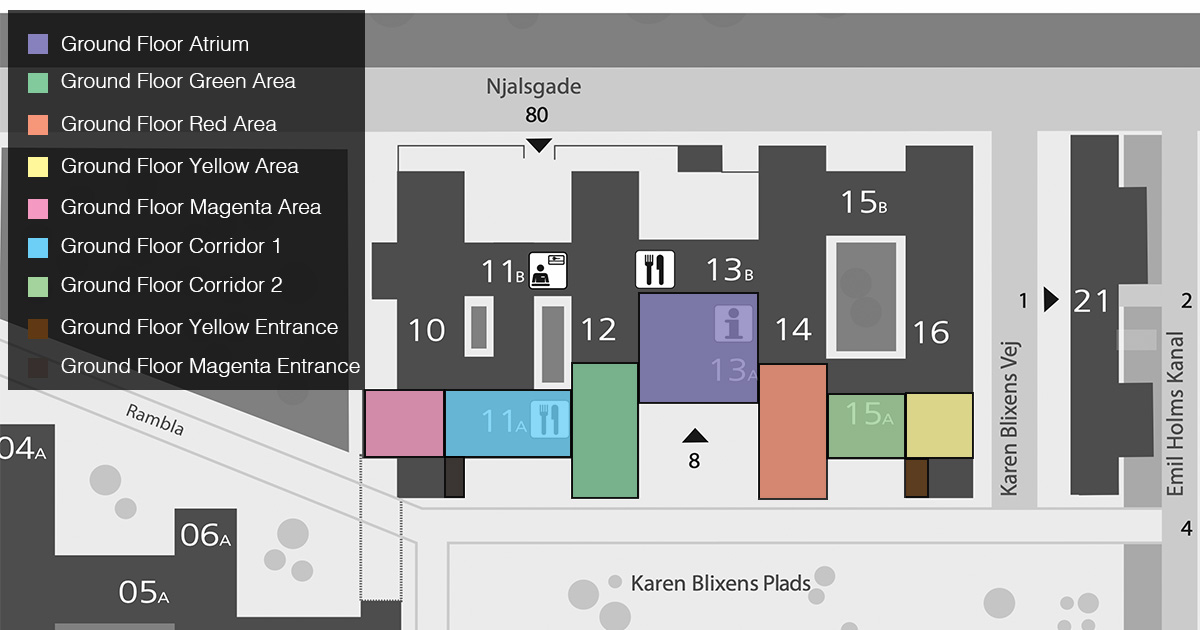
\includegraphics[width=\linewidth]{figures/map-ground-floor.jpg}
      \caption{Ground Floor}
      \label{fig:map-ground-floor}
    \end{subfigure}
    \hfill
    % subfigure
    \begin{subfigure}[b]{0.49\linewidth}
      \centering
      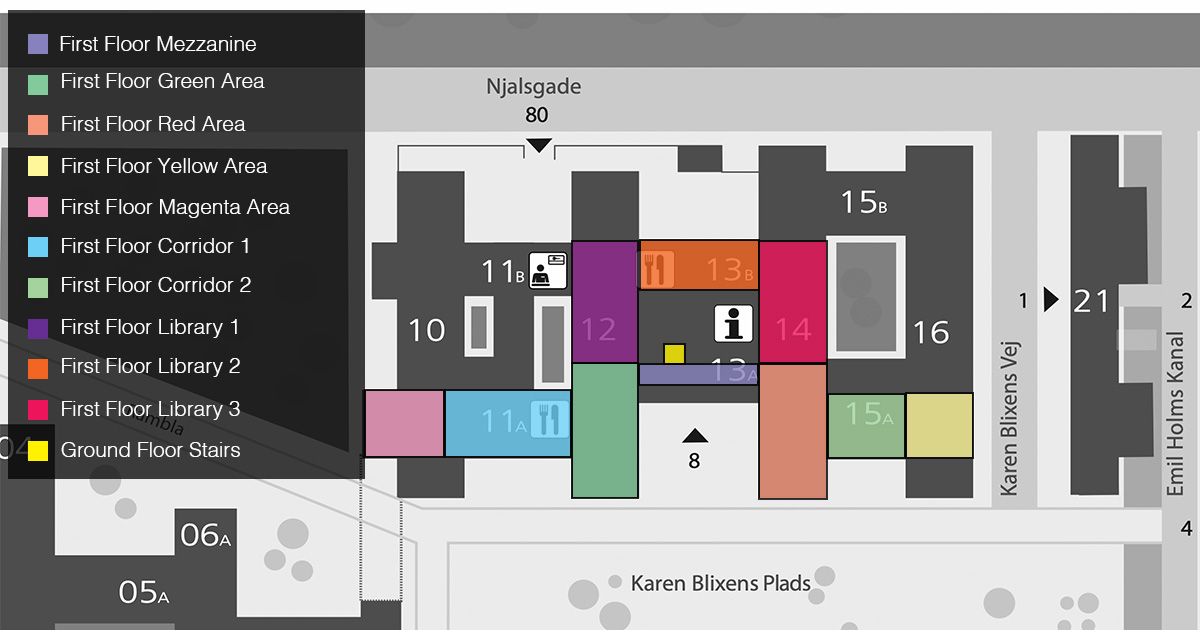
\includegraphics[width=\linewidth]{figures/map-first-floor.jpg}
      \caption{First Floor}
      \label{fig:map-first-floor}
    \end{subfigure}
    \caption{Map of KU Southern Campus Main Building with Location Labels}
    \label{fig:map}
  \end{figure}


  % subsection data-collection (end)

  \subsection{Data Preprocessing} % (fold)
  \label{sub:data-preprocessing}

  The data set was pre-processed to make it suitable for fine-tuning several deep
  learning models. The pre-processing steps broadly involved resizing the video
  footage to a smaller resolution, down-sampling the frame rate, and splitting
  the data set into a training, validation and test set.

  The video footage was resized to a resolution of 224x224 pixels, which is the
  input resolution of most modern foundation models for image and video
  classification, which were used in this project. Furthermore, it decreases the 
  total data amount significantly, which allowed for less disk usage and faster
  loads into memory during training.

  With a similar intention, the video was downsampled to a lower frame rate
  (between 1-5 FPS) to decrease the total data amount. It was hypothesised that
  because of the strong local dependency of consecutive frames, machine learning
  models would heavily overfit to the training footage. Empirical experiments
  confirmed that downsampling indeed reduces the over-fitting, and thus improve
  the robustness of the model against unseen data. The lower frame rate was
  therefore adopted for all further experiments.

  Lastly, the video footage was split into a training, validation and test set,
  based on the date, on which the video footage was recorded. The training set
  only consists of data that was recorded on single days (February \nth{22} 2023
  for the Ground Floor and March \nth{3} 2023 for the First Floor), while the
  validation and testing set consists of data that was recorded on multiple days
  (spanning from \nth{9}-\nth{23} of March 2023). This was a deliberate choice,
  in order to test whether an accurate model could be trained on only a single
  day of footage and still be robust against video clips with vastly different
  lighting conditions, temporal objects, and other factors that could affect the
  model's performance.

  Some examples of frame-location label pairs after preprocessing are shown in
  Figure~\ref{fig:preprocessed-data}.

  % figure
  \begin{figure}[ht]
    \centering
    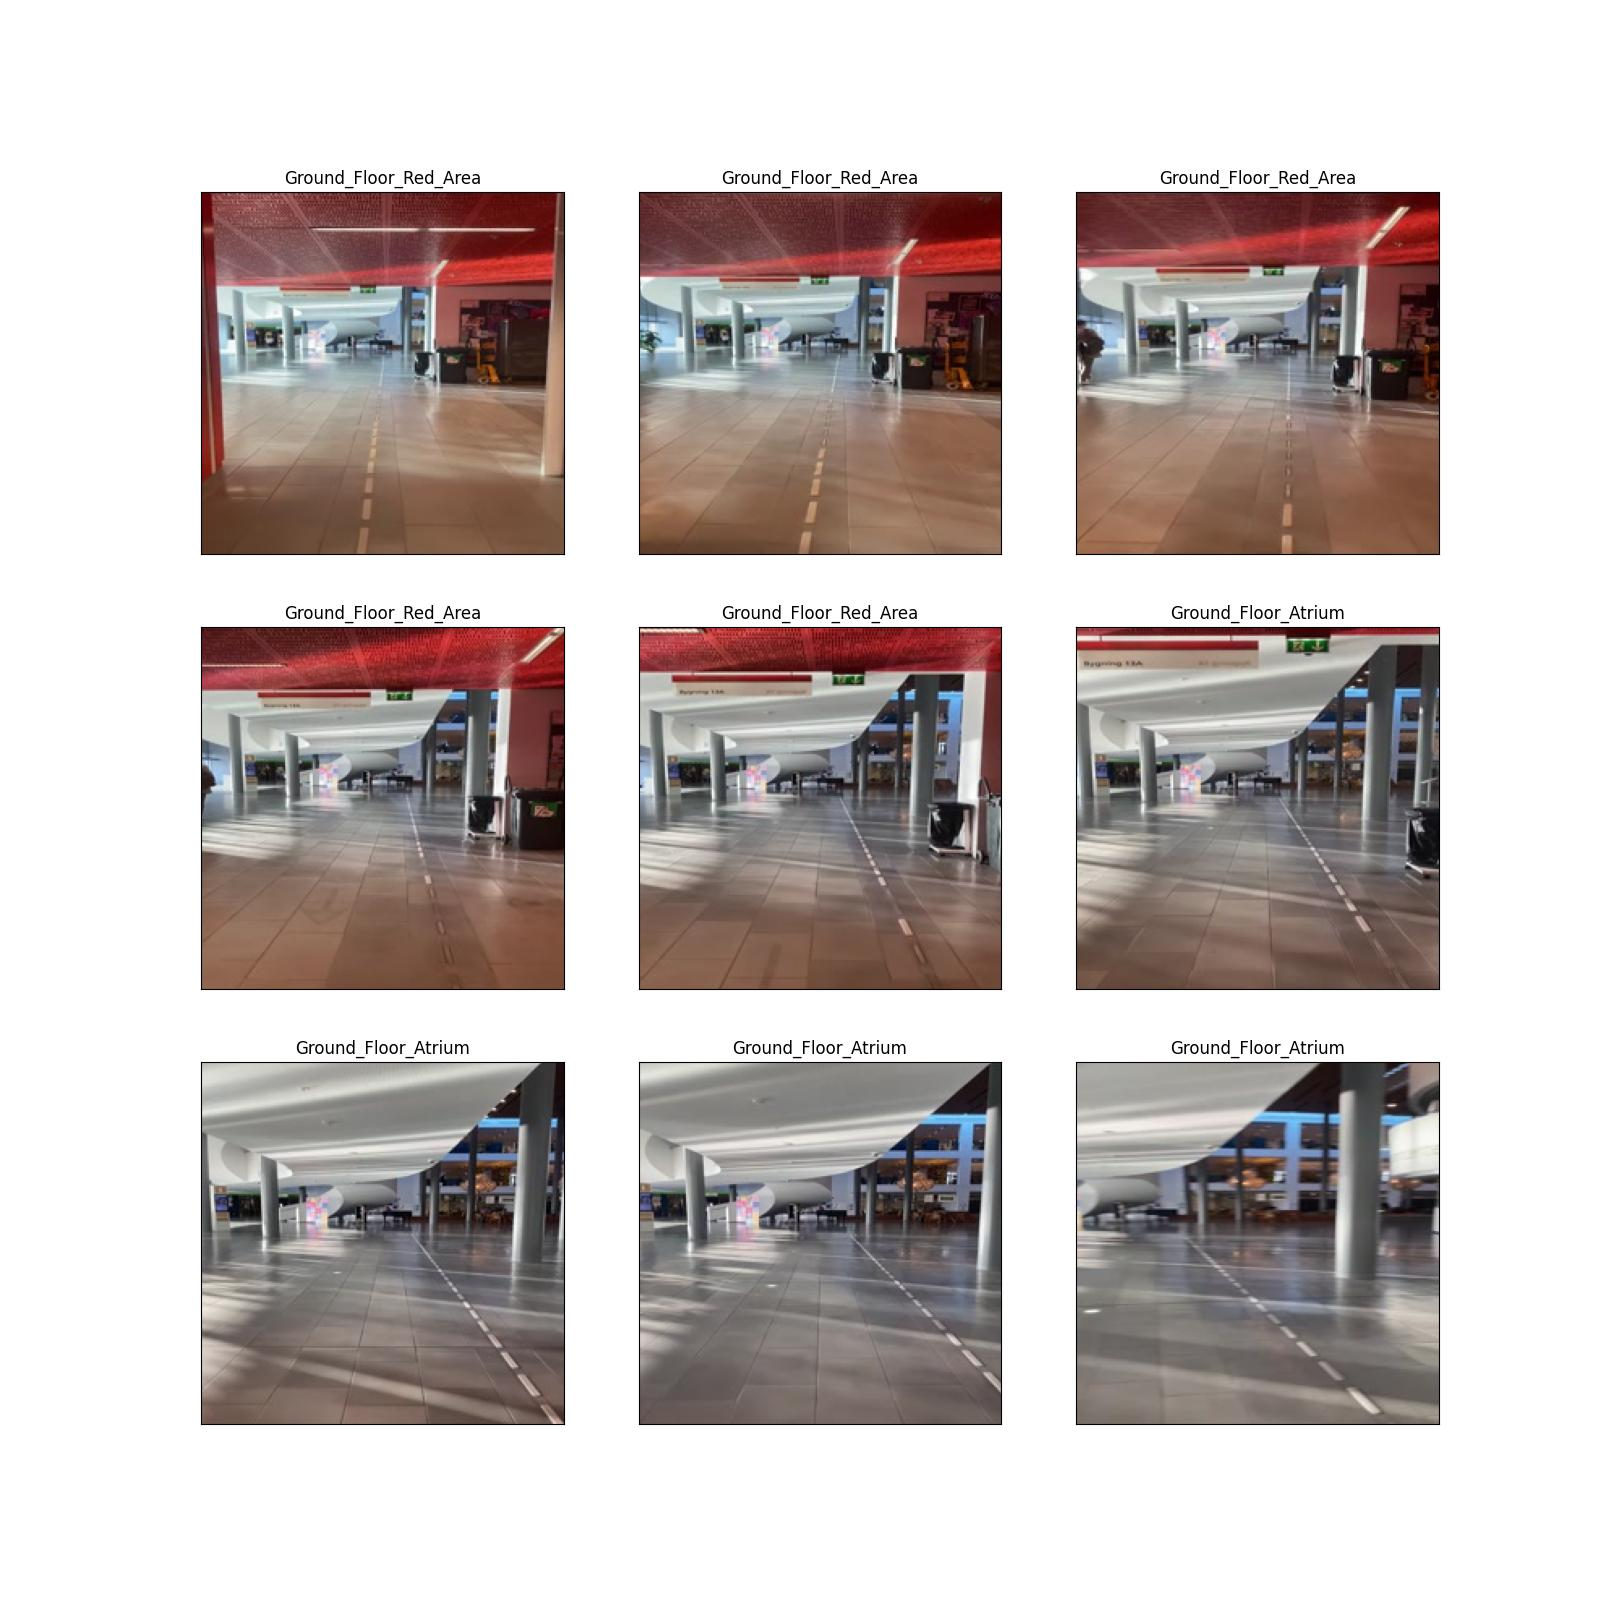
\includegraphics[width=\linewidth]{figures/preprocessed-data.jpg}
    \caption{Examples of preprocessed frame-location pairs}
    \label{fig:preprocessed-data}
  \end{figure}
  
  % subsection data-preprocessing (end)

  \subsection{Models} % (fold)
  \label{sub:models}

  The project uses a fine-tuning approach to train various deep learning model for
  the task of indoor localisation. The fine-tuning approach is a common
  technique in machine learning, where a pre-trained model is used as a starting
  point for training a new model. The pre-trained model is usually trained on a
  large data set, such as ImageNet, and is therefore
  already capable of extracting useful features from images. The pre-trained
  model is then fine-tuned on a smaller data set, which is specific to the
  problem at hand. This approach is advantageous because it allows for the
  training of a model with a relatively small data set, while still achieving
  good performance.

  % subsection models (end)

  \subsection{Experiment Setup} % (fold)
  \label{sub:experiment-setup}

  Here I write something about the experiment setup, like the different
  research questions that I wish to answer and how I aim to test them. Each
  should list precisely which models are trained, under which hyper-parameters,
  and which metrics are used to evaluate the models.

  \begin{enumerate}
    \item Which model architecture performs best? (compare multiple different
      models and test with a set of metrics)
    \item How does the model performance decrease when trained on smaller
      subsets of the data (This is important to assess how little the effort is
      to get a train an initial model that can be deployed)
    \item How does the model performance decrease when trained on a single day
      of data?
  \end{enumerate}
  
  % subsection experiment-setup (end)

  % section methodology (end)

  \section{Results} % (fold)
  \label{sec:results}

  % section results (end)

  \section{Discussion} % (fold)
  \label{sec:discussion}

  % section conclusion (end)

  \section{Conclusion} % (fold)
  \label{sec:conclusion}

  % section conclusion (end)

  % bibliography
  \newpage
  \bibliography{references}
  \bibliographystyle{plain}

\end{document}
